\documentclass{beamer}
\mode<presentation>
\usetheme{Montpellier}

\beamertemplatenavigationsymbolsempty
\pgfdeclareimage[]{logo}{escape-logo}
\logo{
\includegraphics{escape-logo}}

\title{}
\author{Dave Morris, Hendrik Heinl}
\institute{University of Edinburgh, CDS/CNRS}


\begin{document}

\begin{frame}
\titlepage
\end{frame}

\section*{Outline}
\begin{frame}{Outline}
\tableofcontents
\end{frame}

\section{What is the VO?}
\begin{frame}{What is the VO?}
A historical view: The Virtual Observatory (VO) is (or will be), a
\newline
\newline
\centerline{\textbf{comprehensive} set of}
\centerline{\textbf{data} and \textbf{services}}
\centerline{relevant to \textbf{astronomy}}
\centerline{accessible from \textbf{clients} of \textbf{your choice}}
\centerline{\textbf{regardless of where you are} and}
\centerline{\textbf{preserving} products of digital astronomy.}
\end{frame}

\begin{frame}{What it's (actually) not:}

A bundle of software used to work with data in astronomy. 
\newline
\newline
But of course you will find and use VO-client implementations in lots of
software like TOPCAT, Aladin, Splat-VO or PyVO. 

\end{frame}


\section{The challenge}

\begin{frame}{''FAIR''}
There's tens of thousands of data collections somewhere online,
and more should be.

To unlock the treasures hidden there, the data has to be
\begin{itemize}
\item \textbf{F}indable
\item \textbf{A}ccesible
\item \textbf{I}nteroperable
\item \textbf{R}eusable
\end{itemize}
\end{frame}

\section{The IVOA}

\begin{frame}{Standards...}
The IVOA constantly develops new standards and evolves existing ones.
Some of them are well established and well known like Cone Search, SIA,
TAP/ADQL, or SAMP whereas other standards like DataLink or obscore are
not so popular (yet). 

Standards have to be developed though. 

\end{frame}

\begin{frame}{Working Groups and Interest Groups}
There are a lot of working groups within the IVOA and for newcomers it
might be a bit overwhelming to get the overview. Some titles are
selfexplaining, for others an introduction may be necessary. If you are
new to the IVOA, these are most likely groups and sessions you will get
in contact in the next days:
\newline
\newline
The Working Groups are: Applications, Data Access Layer, Data Model,
Grid and Web Services, Resource Registry, and Semantics.
\newline
\newline
The Interest Groups are: Data Curation and Presevation, Education,
Knowledge Discovery, Operations, Radio Astronomy, Solar System, Theory,
and Time Domain.
\end{frame}

 
\begin{frame}{Other groups and Committees}
\begin{itemize}
\item IVOA Executive
\item IVOA Technical Coordination Group
\item IVOA Standing Committee on Science Priorities
\item Standing Committee on Standards and Processes 
\end{itemize}

\end{frame}


\begin{frame}{The Interoperability meetings}

The Interops are rather a working meeting than a conference. Thus,
though many presentations may seem to focus on achievements, they often
are addressed to a specific standard (either established or in
development) and how to improve them. Discussions are much appreciated,
as are reports on caveats or real bugs in the standards: this is how the
VO improves! \newline
\newline
This being said: we encourage you to get involved into the discussions! 


\end{frame}



\section{Demo}

\begin{frame}{Demo time}

Let' see how all this works together.

\end{frame}



\section{Putting it together}

\begin{frame}{All at one glance:}

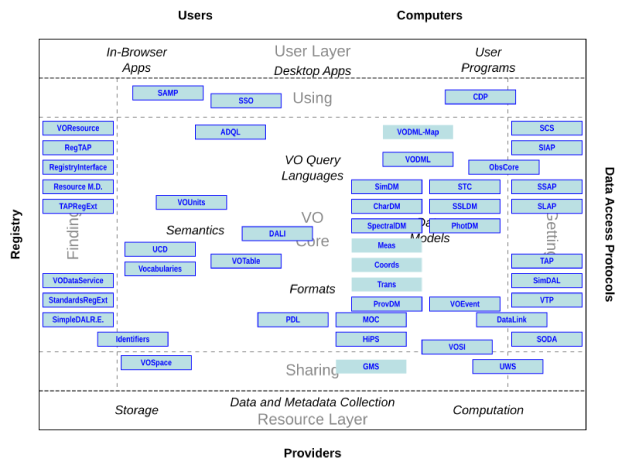
\includegraphics[width=\linewidth]{archdiag2.png}
\end{frame}


\section{This Interop}

\begin{frame}{May 2021 - online}

We thank you for your attention and hopefully we could give you a
helpful preparation to the IVOA Interop meeting. 

See you in way too few hours! 

\end{frame}






\end{document}
